\documentclass{article}
\usepackage{arxiv}

\usepackage[utf8]{inputenc}
\usepackage[english, russian]{babel}

\usepackage[T2A]{fontenc}
\usepackage[utf8]{inputenc}
\usepackage{url}
\usepackage{booktabs}
\usepackage{amsmath}
\usepackage{amsfonts}
\usepackage{nicefrac}
\usepackage{microtype}
\usepackage{lipsum}
\usepackage{lmodern}
\usepackage{graphicx}
\usepackage{natbib}
\usepackage{doi}
\usepackage{algorithm}
\usepackage{algorithmicx}
\usepackage{algpseudocode}
\usepackage{mathtools}
\usepackage{tabularx}

\title{Эффекты самоорганизации в рекомендательных системах}

\author{ Дементьев Сергей \\
        МФТИ\\
	\texttt{dementev.sa@phystech.edu}  \\
	\And
	Веприков Андрей \\
        МФТИ \\
	\texttt{veprikov.as@phystech.edu}  \\
	\And
    Хританков Антон \\
    ВШЭ, МФТИ\\
     \texttt{akhritankov@hse.ru} \\
}
\date{}


\renewcommand{\undertitle}{}
\renewcommand{\shorttitle}{Эффекты самоорганизации в рекомендательных системах}


%%% does not show
%%% DeclareMathOperator*{\norm}{norm}


%%% Add PDF metadata to help others organize their library
%%% Once the PDF is generated, you can check the metadata with
%%% $ pdfinfo template.pdf
%%% \hypersetup{
%%% pdftitle={A template for the arxiv style},
%%% pdfsubject={q-bio.NC, q-bio.QM},
%%% pdfauthor={David S.~Hippocampus, Elias D.~Striatum},
%%% pdfkeywords={First keyword, Second keyword, More},
%%% }


\begin{document}
\maketitle


\begin{abstract}
    В работе исследуются петли скрытой обратной связи в рекомендательных системах.
    Решается задача поиска условий возникновения положительной обратной связи. Исследуется эффект самоорганизации в рекомендательной системе, в которой "товары" и "пользователи" меняются со временем.
\end{abstract}


\keywords{Петли обратной связи \and Рекомендательные системы \and Контролируемое машинное обучение}


\section{Введение}


Рекомендательные системы, формирующие пользовательский опыт на таких платформах, как YouTube, Netflix и социальные сети, играют ключевую роль в цифровой экосистеме, определяя, какой контент достигает аудитории. Однако их способность усиливать вовлечённость пользователей зачастую приводит к нежелательным последствиям, включая формирование эхо-камер и фильтрующих пузырей, которые ограничивают разнообразие информации и усиливают социальную поляризацию. Скрытые петли обратной. 
связи, возникающие, когда рекомендации изменяют поведение пользователей, а изменённые данные влияют на последующие алгоритмы, представляют серьёзную угрозу безопасности цифровых систем [1]. Обеспечение безопасности рекомендательных систем
требует выявления и предотвращения таких петель, чтобы защитить пользователей от
манипуляций, сохранить этичность алгоритмов и поддерживать доверие к платформам.
Петли обратной связи создают множество рисков для безопасности. Во-первых, эхокамеры, формируемые алгоритмами, усиливающими существующие предпочтения, могут радикализировать пользователей, ограничивая их доступ к разнообразным точкам
зрения и усиливая дезинформацию [3]. Например, гиперактивные пользователи, чьи действия непропорционально влияют на тренды, могут искажать рекомендации, создавая
замкнутые циклы, где контент адаптируется под узкие интересы, угрожая информационной безопасности [2]. Во-вторых, злонамеренные агенты могут использовать уязвимости систем, искусственно продвигая контент через поддельные аккаунты, что подрывает целостность платформы и создаёт риски манипуляции общественным мнением [4].


Эти угрозы подчёркивают необходимость разработки безопасных алгоритмов, способных минимизировать влияние петель обратной связи.
В данной работе мы рассматриваем рекомендательные системы как динамические
системы, где предпочтения пользователей и характеристики товаров эволюционируют
под воздействием алгоритмов рекомендаций. Основываясь на математической модели
из [1], мы исследуем механизмы формирования эхо-камер, определяемых как слабая сходимость распределений предпочтений пользователей к смеси дельта-функций. Такой
подход позволяет формально анализировать условия, при которых системы становятся
уязвимыми, и предлагать стратегии повышения их безопасности. Наша цель — разработать теоретические и практические инструменты для отслеживания и предотвращения
эхо-камер, обеспечивая устойчивость и безопасность рекомендательных систем в условиях скрытых петель обратной связи


В своей статье мы представляем несколько критериев, для выявления эхо-камеры, которые будут полезны не только специалистам в машинном-обучении, но и социологам : 

1) Эхо-камера – это ситуация, при которой функция распределения пользователей сходится слабо к смеси дельта-функций: $f_{U_t} \underset{t\rightarrow \infty}{\rightharpoonup} \sum_{i=1}^K w_i \delta_{u_i}$, где K – количество получившихся "эхо-камер" в системе. А $u_i$ нужно понимать как центр этого кластера (То есть, это портрет среднего пользователя в данной группе)

2) Необходимое и достаточное условие существование Эхо-камеры дает теорема I, при этом, на практике, можно проверять только свойство $\lambda (HDR_{\alpha} (f_{U_t}) ) \rightarrow 0$, где $\lambda$ – мера Лебега на $\mathbb{R}^n$, а $HDR$ (High Density Region) $= \{x\in \mathbb{R}^n | f(x) \geq c_\alpha \}, $ где $c_{\alpha} = \sup \{ c |  \lambda (x \in HDR_{\alpha}(f) ) \geq \alpha  \}$ 



\section{Related Work}
На данный момент нет единого определения что такое петля. 

Приведу несколько определений и затем мы проанализируем, как они соотносятся: 

1) Согласно Wang et al. \cite{wang2025decoding}, эхо-камеры возникают, когда люди в основном подвергаются воздействию информации или мнений, которые соответствуют их собственным, что ограничивает их знакомство с разнообразными точками зрения и усиливает существующие убеждения.

В своей работе, они исследовали их возникновение с помощью нескольких метрик. 

NCI (normalized clustering index), DG (глобальное недовольство), Pz (поляризация)

2) В исследовании 2024 года \cite{mehrabi2024flirt}, посвященному возникновению скрытых петель в системах с большими языковыми моделями, авторы считают, что использование выхода модели – уже дает возможность полагать, что возникла петля обратной связи. 

3) В статье \cite{breaking_feedbackloops2022} в рекомендательных системах формулируются как циклический процесс, в котором рекомендательная система влияет на данные о поведении пользователей, которые затем используются для обновления этой же системы.

Математически это выражается через нарушение независимости между наблюдениями в разные моменты времени. Ключевая формула, которая показывает наличие петли обратной связи, выражается уравнением:

$P(\{ R_s \}_{s=1}^t | \{ A_s\}_{s=1}^t) = \prod\limits_{s=1}^t P(R_s | A_s, \{R_{s'}, A_{s'} \}_{s'=1}^{s-1}) \neq \prod\limits_{s=1}^t P(R_s | A_s)$

Эта формула показывает, что совместное распределение рейтингов пользователей ($R$) при заданных рекомендациях ($A$) не распадается на произведение независимых распределений. Если левая и правая части этого уравнения не равны друг другу, это указывает на наличие петли обратной связи в системе рекомендаций.

В отсутствие петель обратной связи рейтинги в разные моменты времени были бы условно независимы при заданных рекомендациях. Неравенство показывает, что рейтинги на самом деле зависят не только от текущих рекомендаций, но и от всей предыдущей истории рекомендаций и рейтингов.

4) Также стоит отметить, что применительно к рекомендательным системам, можно дать следующее определение эхо-камере на "языке социологов"

Эхо-камера — это среда или экосистема, в которой участники сталкиваются с убеждениями, которые усиливают или подкрепляют их уже существующие убеждения посредством общения и повторения внутри закрытой системы и изолированы от опровержения. Эхо-камера распространяет существующие взгляды, не сталкиваясь с противоположными взглядами, что может привести к предвзятости подтверждения. Эхо-камеры могут усиливать социальную и политическую поляризацию и экстремизм. В социальных сетях считается, что эхо-камеры ограничивают воздействие различных точек зрения и способствуют и усиливают предполагаемые нарративы и идеологии.


Рассмотрев такие разные определения, сформулированные с применением аппарата из различных областей математики, что на данный момент четкого понимания, что же такое петля обратной связи. Но это не так, уже есть понимание, что петля обратной связи – это свойство системы. Оно не может быть измерено в определенный момент времени. Для понимания петли обратной связи, нужно исследовать полностью эволюцию системы. 


\section{Постановка задачи}

Мы дадим определение эхо-камере, согласовав его с определением, пришедшим к нам от социологов. Имея математическое определение эхо-камеры, мы сможем построить математическую модель возникновения петли и используя введенные нами определения, формально отследить, когда возникает петля. Это позволит нам исследовать возникновение эхо-камер в рекомендательных системах в зависимости от различных параметров модели. 


Возникновение эхо-камеры – это прямое следствие появления петли обратной связи в нашей системе. Мы будем считать, что наша система состоит из: 

\renewcommand{\labelitemi}{•} 
\begin{itemize}
    \item $I$ – множество товаров (items), которые будут рекомендоваться.

    
    \item  $U$ – множество пользователей (users), они будут взаимодействовать с рекомендациями от нашего алгоритма. 

    \item $R$ – отображение вида, $R : U \times I \rightarrow \mathbb{R}$, которое сопоставляет паре $($пользователь, товар$)$ оценку, в конечномерном случае, $R$ можно понимать как матрицу, $R \in \mathbb{R}^{|U| \times |I| }$

    \item $D_t = (U_t, I_t, R_t)$ – датасет, именно такие данные будут подаваться нашему алгоритму обучения 

    \item $f_U, f_I$ – функции распределения пользователей и товаров. В данной модели, мы предполагаем, что эти функции измеримые, они существуют в каждый момент времени и ограничены. 
    
    \item $\mathbf{D}_t$ – эволюционное отображение, введенное аналогично статье \cite{veprikov2024mathematical}.
    $\mathbf{D}_t: \mathbf{F} \rightarrow \mathbf{F}$, где 
    $\mathbf{F} := \big\{ f: \mathbb{R}^n \rightarrow \mathbb{R}_{+} | \int_{\mathbb{R}^n} f(x) dx = 1  \big\}$ – то есть множество всех функций, которые могут быть плотностью некоторого случайного вектора. 

    Отображение эволюции важно тем, что оно задает очень важное рекурентное соотношение: 
    
    $$\mathbf{D}_t f_t = f_{t+1} \quad\forall t \in \mathbb{N}$$, 

\end{itemize}
В данной работе у нас есть множество пользователей $U$ (users) и товаров $I$ (items), эти множества не наделены никакой структурой, для постановки и решения задачи мы перейдем к $E_U$ и $E_I$ – евклидовым пространствам, в которые переводятся множества $U$ и $I$, с помощью инъективных отображений $\phi_U $ и $\phi_I$ (эти функции сопоставляют каждому пользователю его "эмбеддинг"). Но в дальнейшем, мы будем опускать написание этих отображений и отождествлять пользователя $u \in U$ и эмбеддинг, представляющий пользователя $e_u \in E_U \subset \mathbb{R}^d$

В данной работе мы не будем исследовать поведение остатков модели, так как в отличие от \cite{veprikov2024mathematical} у нас задача многомерная и определить последовательность остатков – затруднительно. 

Мы хотим исследовать поведение системы из пользователей и товаров с течением времени $t$, поэтому большинство величин имеет индекс $t$. Так как мы рассматриваем нашу модель как динамическую систему, то в каждый момент времени мы будем иметь $D_t$ – датасет. Он будет использоваться для обучения всех алгоритмов на шаге $t$, а также валидации нашей модели. 


Мы исследуем, когда при использовании последовательности отображений эволюций могут возникнуть эхо-камеры. Дальше мы будем отождествлять "оператор эволюции" и "отображение эволюции", хотя, очевидно, что $\mathbf{D}_t$ – не обязательно линейное отображение и не обязательно отображение между линейными пространствами, но аналогично операторам, мы можем ввести норму отображения

$||\mathbf{D}|| := \underset{||x||=1}{\sup} ||\mathbf{D}x||$, и сузить класс возможных операторов эволюций.

\textbf{Определение:} Мы будем говорить, что в динамической системе, которая характеризуется начальными данными: $D_{1} = (U_1, I_1, R_1)$, последовательностью операторов эволюции: $\{\mathbf{D}_t \}_{t=1}^{\infty}$ возникли эхо-камеры, если существует конечное множество точек $\{u_1, \ldots u_K \} \subset \mathbb{R}^d, K \geq 1$ и соотвествующие веса $\{w_1, \ldots w_K \}, \sum_{i=1}^K w_i = 1$, такие что: 

 $$f_t \underset{t\rightarrow \infty}{\rightharpoonup} \sum_{i=1}^K w_i \delta_{u_i}$$ (слабо сходится к смеси дельта-распределений)

 


\section{Теоретические результаты}

Введем отображение $HDR_{\alpha} (f)$ для некоторого $\alpha \in [0;1]$, которое функции, сопоставляет множество с наибольшей плотностью, и контроллируемой суммарной вероятностью этого множества. Более формально: 

$HDR_{\alpha}(f) $= \{x\in \mathbb{R}^n | f(x) \geq c_\alpha \}, $ где $c_{\alpha} = \sup \{ c |  \lambda (x \in HDR_{\alpha}(f) ) \geq \alpha  \}$ 

Тогда мы можем сформулировать теорему, которая позволит нам отслеживать возникновение эхо-камер



\textbf{\underline{Теорема I (критерий возникновения эхо-камеры) : } }



Пусть $\{ f_t \}_{t=1}^{\infty}$ – последовательность функций плотности распределений в пространстве признаков $\mathbb{R}^d$. Эхо-камера формируется в системе тогда и только тогда, когда существует уровень $\alpha_0 \in (0; 1)$ такой, что для любого $\alpha < \alpha_0$ выполняются следующие условия: 

1. $\exist K \in \mathbb{N}$ и момент времени $T_0$, такие что $\forall t > T_0:$ множество $HDR_{\alpha}(f_t)$ состоит ровно из $K$ компонент. $HDR_{\alpha}(f_t) = \cup_{i=1}^K C_{i, t}$


2. $\exists \delta > 0, T_0 $ такое, что $\underset{i \neq j}{\min} d(C_{i, t}, C_{j, t}) \geq \delta  \quad \forall t > T_0$

Где $d(A, B) = \underset{x \in A, y \in B}{\inf} ||x - y||$

3. $\lim\limits_{t \rightarrow \infty} \lambda \big( HDR_{\alpha} (f) \big) = 0$

4.  


\textbf{\underline{Обсуждение теоремы I:}} не смотря на свою громоздкость, условия, которые появляются в этой теореме – не слишком обременительны. Это лишь логичные предположения о возникновении эхо-камеры. Пункт 1 означает в какой-то момент времени произойдет стабилизация компонент и множество повышенной плотности будет состоять только из конечного числа компонент, к которым и будут сжиматься распределения. При этом, не исключено, что это число может быть равным одному $K = 1$, либо $K = |U|$ это может сигнализировать нам о том, что  в системе очень мало людей. 


В пункте 2 речь идет о том, что в какой-то момент времени кластеры можно различить. Причем это условие тоже может легко выполняться, так как мы вольны выбирать $\alpha_0$ сколь угодно близкой к 0. 

Ну и самый важный пункт – пункт 3, который говорит о том, что мера множеств составляющих кластер – стремится к нулю со временем. 

При этом, можно центры кластеров – $\ {u_i \}_{i=1}^K$ – могут быть различными характеристиками от кластеров. Но можно провести аналогию с тем, что $u_i$ – показывает среднего пользователя в $i-$ом кластере. 


При этом, мы будем отслеживать в каждый момент времени $HDR_{\alpha}(f_t)$ и на основе этого определять – возникла ли эхо-камера или нет. 


При этом, аналогично теореме, задающей границу на скорость сходимость ошибки \cite{veprikov2024mathematical} можно построить аналогичную теорему: 

\textbf{ \underline{Теорема II (критерий возникновения петли обратной связи): } }


Пусть $f_1 \in \mathbf{F}$ – некоторая начальная функция плотности. Если существуют точки $\{u_1, \ldots u_K \}$ и веса $\{w_1, \ldots w_K \}, \sum_{i=1}^K w_i = 1$, измеримые функции $\{g_1, \ldots g_K \} \subset L_1(\mathbb{R})$ и неотрицательные последовательности $\{\psi_{1, t}, \ldots \psi_{K, t} \}$ такие, что: 

$$f_t(u) \leq \sum_{i=1}^K w_i (\psi_{i, t})^m |g_i(\psi_{i, t} \cdot (u - u_i)) | \quad \forall u \in \mathbb{R}^d, t \in \mathbb{N}$$

И если: 

1) $\forall i \psi_{i, t} \underset{t \rightarrow \infty}{\rightarrow} \infty, $ то: $f_t \rightharpoonup \sum_{i=1}^K w_i \delta_{u_i}$


2)  $\forall i \psi_{i, t} \underset{t \rightarrow \infty}{\rightarrow} 0,     $ то: $f_t \rightharpoonup \zeta$ (нулевое распределение)


3) Пусть $I \subset \overline{\{1, 2, \ldots K \}}$ и если 

$\forall i \in I: \psi_{i, t} \rightarrow \infty $ и $\forall j \in \overline{\{1, 2, \ldots K}}  \} \setminus I : \quad \psi_{j, t} \rightarrow 0$, то $f_t \rightharpoonup \sum_{i \in I}w_i \delta_{u_i}$

\underline{Обсуждение теоремы II: }


В данном случае мы получаем оценку на скорость сходимости системы к эхо-камере. Что может подтолкнуть нас на более чувствительный критерий определения наличия петли в системе. 

$\lambda(HDR_{\alpha}(f_t)) \sim \sum\limits_{i=1}^K \frac{1}{\psi_{i, t}^m}, \quad t\rightarrow \infty$





 
\section{Метод}



В нашей рекомендательной системе действует алгоритм рекомендаций $a_{rec}(u, i, \theta)$ – это отображение сопоставляет пользователю $u$ и товару $i$ число из интервала $[0; 1]$, которое характеризует вероятность взаимодействия пользователя с товаром. $a_{rec}$ зависит также от $\theta$ – некоторых латентных параметров, которые вносят стохастичность в нашу динамическую систему. При этом, можно определить с помощью $a_rec$, $A_t$ – рекомендации на шаге $t$ для всех пользователей в системе. Например, мы для каждого пользователя и для каждого товара смотрим $a_{rec}(u, i)$ и для каждого пользователя оставляем только топ-$K$ самых подходящих товаров. 

Также у нас есть алгоритм $a_{choice}$ – алгоритм выбора товара. Это отображение вида $U \times I^K \rightarrow I  \cup \{ \emptyset \}$, которое сопоставляет паре $(u, (i_1, i_2, ... i_K))$ , состоящей из пользователя $u$ и кортежа $(i_1, ... i_K)$ (которые далее будут интерпретироваться как порекомендованные товары), выбор из этих рекомендованных товаров, либо вообще не рекомендовать товар. Эта функция будет имитацией выбора товара пользователем, после предложения рекомендации алгоритмом $a_{rec}$. 

Также у нас есть два алгоритма $a_{u'}$ и $a_{i'}$ – эти два алгоритма привносят в нашу динамическую систему новые товары и новых пользователей. Формально это лишь отображения из множества $\mathscr{D}_t$ в $E_U$ или $E_I$. Помимо этого, эти алгоритмы могут убирать объекты из системы. Например, таким образом, моделируется уход пользователя, которому долго ничего не нравилось




\begin{algorithm}
\caption{Модель рекомендации для детекции петли обратной связи}\label{one_exp}
\begin{algorithmic}[1]
\State $T \gets 100$ \Comment{ограничение на количество итераций }
\While{$t  < T $}\Comment{пока не дошли до ограничения по времени}
\State $a_{rec} \gets \text{train}(D_t^*)$ \Comment{тренируем модель рекомендаций, ей не доступна вся информация}
\State $a_{choice} \gets \text{train}(D_t)$\Comment{тренируем модель выбора пользователей, ей доступна вся информация}

\State $A_t \gets \text{pick up recommendations}(a_{rec}, D_t)$ \Comment{подбираем рекомендации}
\State $R_{t+1} \gets \text{respond to recommendations}(a_{choice}, D_t)$\Comment{Моделируем ответы пользователей на рекомендации}
\State $U_{t+1} \gets a_{u'}(D_t)$ \Comment{Обновляем пользователей}
\State $I_{t+1} \gets a_{i'}(D_t)$ \Comment{Обновляем товары}

\State $D_{t+1} \gets (U_{t+1}, I_{t+1}, R_{t+1})$ 
\State $D_{t+1}^* \gets (\text{proj}(U_{t+1}, dims), \text{proj}(I_{t+1}, dims), R_{t+1})$ \Comment{Сохраняем датасет с неполной информацией, чтобы на нем обучить $a_{rec}$}
\EndWhile

\end{algorithmic}
\end{algorithm}


При этом, в нашей системе есть множество параметров, которые зависят друг от друга сложным образом и которые непосредственно влияют на систему. Самые основные (по степени непосредственного влияния) выписаны в таблице ниже: 


\begin{center}
\setlength{\tabcolsep}{12pt}
\renewcommand{\arraystretch}{1.8}

\begin{tabularx}{\textwidth}{|c|>{\raggedright\arraybackslash}X|}
\hline
$\dim(E_U), \dim(E_I)$ & размерность эмбеддинга пользователей и товаров  \\ \hline
$\dim(E_U^{rec}), \dim(E_I^{rec})$ & размерность эмбеддингов пользователей и товаров, которые будут подаваться в модель $a_{rec}$ \\ \hline
$\dim(E_U^{choice}), \dim(E_I^{choice})$ & размерность эмбеддингов пользователей и товаров, которые будут подаваться в модель $a_{choice}$ \\ \hline
$\varphi_I^{rec}, \varphi_{U}^{rec}$ & отображения, которые понижают размерность изначального пространства эмбеддингов. (Это может быть как PCA, t-SNE, так и просто взятие первых $\dim(E^{rec})$ координат от начального вектора) \\ \hline
$\varphi_I^{rec}, \varphi_{U}^{rec}$ & отображения, которые понижают размерность изначального пространства эмбеддингов. (Это может быть как PCA, t-SNE, так и просто взятие первых $\dim(E^{rec})$ координат от начального вектора) \\ \hline
$K$ & количество рекомендаций, предлагаемых определенному пользователю \\ \hline
$\mathcal{P}_U, \mathcal{P}_I$ & Параметризованное семейство распределений, которое задает распределение эмбеддингов пользователей и товаров  \\ \hline
$T_{rec}, T_{choice}$ & период, в течение которого модель рекомендаций / выбора пользователей не обновляется \\ \hline
$\mathcal{A}_{\text{emb}}$ & семейство алгоритмов оптимизации для получения эмбеддингов пользователей из начальных данных по сделкам (т.е. алгоритм для колаборативной фильтрации) \\ \hline
$\mathcal{A}_{\text{train}}$ & алгоритм оптимизации для обучения модели $a_{rec}, a_{choice}$ \\ \hline
$\Theta_{\text{emb}}$ & параметры модели, с помощью которой мы получили эмбеддинги \\ \hline
$\Theta_{\text{rec}}, \Theta_{\text{choice}}$ & гиперпараметры моделей $a_{rec}$ и $a_{choice}$ (например, в случае полносвязных нейронных сетей – это количество скрытых слоев и нейронов в них) \\ \hline
\end{tabularx}
\end{center}

\section{Вычислительный эксперимент}

\subsection{Описание данных}

В качестве данных мы используем MovieLens 100K movie ratings.


\subsection{Модель}



Используется следующая модель: 
\begin{center}
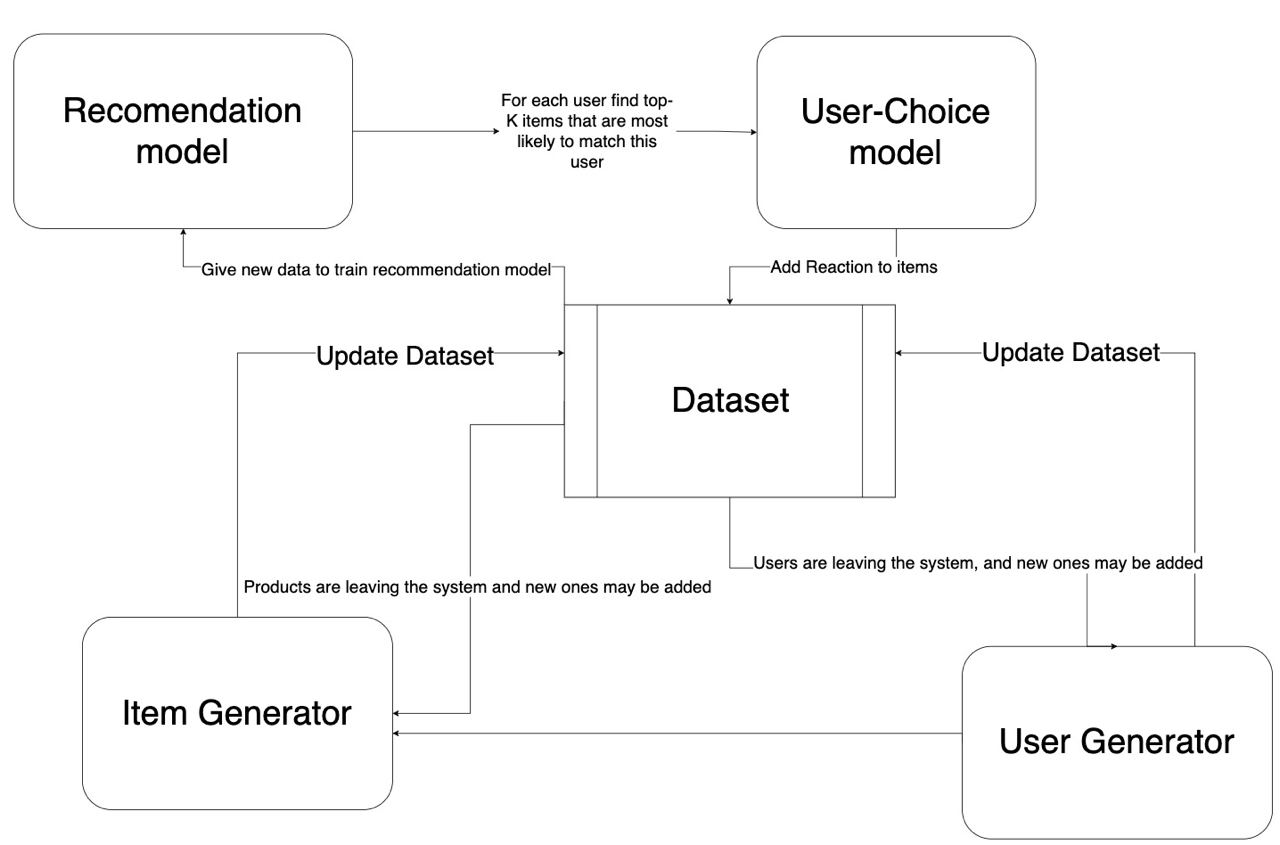
\includegraphics[width=0.7\textwidth]{model.jpg}
\end{center}

В качестве $a_{rec}$ мы используем нейронную двуслойную сеть с одной функцией активации. Аналогично с $a_{choice}$. Но в ходе эксперимента $a_{choice}$ обучается только лишь с некоторой периодичностью.  

В начальный момент времени мы возьмем выходы некоторой нейронной сети. И критерием того, что эмбеддинги подходят для представления пользователей – это их нормальность. (Она проверяется отдельно с помощью МПГ и теста Колмогорова-Смирнова). Причем, в каждый момент времени мы будем оценивать матрицу ковариации и вектор средних для пользователей, оставшихся в системе. Это и будет параметрами многомерного нормального распределения из которого мы будем генерировать новых пользователей и новые товары.


Также важно отметить, что вычисление $HDR$ по выборке – отдельная задача вычислительной математики. А так как мы имеем дело со сложными мультимодальными распределениями, носитель которых может быть множеством с большой размерностью, то важно оценивать $HDR$ максимально эффективно по времени и качеству оценки. 

Пусть $X$ – выборка из $n$ элементов, по которой мы хотим оценить $HDR$, $X \subset \mathbb{R}^d$, $k$ – параметр алгоритма оценки $HDR$, который будет пониматься как число соседей в вычислении $kNN(x, X)_{j}$ – $j-$ого ближайшего соседа из выборки $X$ для элемента $x$. Если $x\in X$, то считаем, что $kNN(x, X)_{1} = 0$, хотя как показано в \cite{kNN_estimate}, на асимптотические свойства дальнейших оценок это не будет влиять. 

Предложенный ниже метод вычисления оценки $\widehat{HDR}$ основан на \cite{HDR_estimate} и об асимптотических свойствах $kNN$ оценки плотности распределения: $f_{kNN}(x) = \frac{1}{Z} \frac{k / n}{ V_k(x)}$, где $V_k(x) $ – объём наименьшей $d-$мерной сферы, с центром в $x$ и которая содержит не менее $k$ точек из $X \setminus \{ x \}$

Тогда можно ввести меру "разреженности" между точками, и тогда области с высокой разреженностью будут областью с низкой плотностью. Более формально: $M(x, X, k) := \sum_\limits{j=1}^K ||x - kNN(x, X)_{j} ||_2$ – мера разреженности. 

Тогда можно посчитать для каждой точки $x \in X$ $M(x, X, k)$, составить из этих значений вариационный ряд, и определить $M^* = M_{(\lceil  \alpha \cdot n \rceil)}$ Тогда 

$$\widehat{HDR} = \{x \in \mathbb{R}^{d} | M(x, X, k) \leq M^*\}$$

А меру этого множества можно оценить методом Монте-Карло и алгоритм примет вид: 


\begin{algorithm}
\caption{Алгоритм вычисления $\lambda(HDR)$}\label{one_exp}
\begin{algorithmic}[1]


\State $k \gets \lfloor\sqrt{n} \rfloor$ \Comment{экспериментальная оценка для $k$ }

\For{$i \gets 1$ \textbf{to} $n$}
    \State $M_i \gets M(X_i, X, k)$
\EndFor

\State $M^{*} \gets M_{(\lceil \alpha \cdot n \rceil)}$ \Comment{определяем константу для $\widehat{HDR}$}



\State $B \gets \prod_{j = 1}^{d}
[\underset{{i\in \{1..n \}}}{\min}( X_i(j)) ; \underset{{i\in \{1..n \}}}{\max}( X_i(j))]$
\Comment{оцениваем носитель распределения}

\State $y_1, y_2, \ldots y_l \sim U(B)$
\Comment{семплируем из равномерного распределения для метода Монте-Карло}


\State $\lambda(HDR) = \frac{\sum_{j=1}^l [M(y_j, X, k) \leq M^* ]}{l} \lambda(B)$


\State \Return $\lambda(HDR)$


\end{algorithmic}
\end{algorithm}

Стоит отметить, что для оценки Монте-Карло следует брать $l = O(n)$, а скорость сходимости этого алгоритма будет порядка $\frac{1}{\sqrt{n}}$. При этом, на практике можно улучшить этот алгоритм, предварительно выделив из множества $\{x \in X | x \in \widehat{HDR}\}$ кластеры, например, с помощью метода DBSCAN, и улучшить дисперсию оценки. Также, предложенный метод вычисления $HDR$ позволяет избежать проклятия размерности \cite{dim_curiosity}.


\subsection{Результаты}

Таблица со степенью влияния: 

\begin{tabularx}{\textwidth}{|c|>{\raggedright\arraybackslash}X|}
\hline
$\dim(E_U), \dim(E_I)$ & ?  \\ \hline
$\dim(E_U^{rec}), \dim(E_I^{rec})$ & ? \\ \hline
$\dim(E_U^{choice}), \dim(E_I^{choice})$ & Влияет, только отношение этих размерностей к размерностям эмбеддингов для модели рекомендаций \\ \hline

$\varphi_I^{rec}, \varphi_{U}^{rec}$ & Чем больше отображение сохраняет инфомрации – тем медленее произойдет появление эхокамеры \\ \hline


$K$ & Если это число большое или маленькое, то можно увидеть очень быструю сходимость \\ \hline
$\mathcal{P}_U, \mathcal{P}_I$ & Рассматривали только смеси нормальных распределений  \\ \hline
$T_{rec}, T_{choice}$ & Чем ближе к единице отношение $T_{rec} / T_{choice}$ \\ \hline

$\mathcal{A}_{\text{emb}}$ & при получении алгоритмов с помощью SGD сходимость была более быстрой к петле, нежели чем с Adam \\ \hline
$\mathcal{A}_{\text{train}}$ & Чем быстрее скорость сходимость метода, тем быстрее получалась петля \\ \hline
$\Theta_{\text{emb}}$ & Менее глубокая сеть дает более быструю сходимость \\ \hline
$\Theta_{\text{rec}}, \Theta_{\text{choice}}$ & ? \\ \hline
\end{tabularx}
\end{center}
После запуска эксперимента мы получили, что петля образуется тем быстрее, чем меньше информации доступно алгоритму $a_{rec}$. 

\begin{center}
\includegraphics[width=0.7\textwidth]{videoframe_0.png}
\end{center}

\begin{center}
\includegraphics[width=0.7\textwidth]{videoframe_1.png}
\end{center}

\begin{center}
\includegraphics[width=0.7\textwidth]{metrics.png}
\end{center}


\begin{center}
\includegraphics[width=0.7\textwidth]{kl_divergence.png}
\end{center}


\section{Заключение}



\begin{thebibliography}{10}


\bibitem{veprikov2024mathematical}
Veprikov, A., et al. A Mathematical Model of the Hidden Feedback Loop Effect in Machine Learning Systems. \url{https://arxiv.org/abs/2405.02726}, 2024.


\bibitem{hidden_simulation}
Hidden Feedback Loops in Machine Learning Systems: A Simulation Model and Preliminary Results. \url{https://link.springer.com/chapter/10.1007/978-3-030-65854-0_5}, 2021.


\bibitem{analysis_hidden}
Analysis of hidden feedback loops in continuous machine learning systems. \url{https://www.researchgate.net/publication/348487258_Analysis_of_hidden_feedback_loops_in_continuous_machine_learning_systems}, 2021.


\bibitem{classification_feedback}
A Classification of Feedback Loops and Their Relation to Biases in Automated Decision-Making Systems. \url{https://dl.acm.org/doi/fullHtml/10.1145/3617694.3623227}, 2023.


\bibitem{pariser2011filter}
Pariser, E. The Filter Bubble: How The New Personalized Web Is Changing What We Read And How We Think. Penguin Books, 2011.


\bibitem{bakshy2015exposure}
Bakshy, E., et al. Exposure to ideologically diverse news and opinion on Facebook. Science, 2015.


\bibitem{matz2017psychological}
Matz, S.C., et al. Psychological targeting as an effective approach to digital mass persuasion. Proceedings of the National Academy of Sciences, 2017.


\bibitem{haimson2021impact}
Haimson, O., et al. The impact of algorithmic personalization on user behavior. ACM Transactions on Interactive Intelligent Systems, 2021.


\bibitem{devreeze2020dynamics}
De Vreeze, J.H., et al. The dynamics of algorithmic filtering: A computational model. Information Systems Research, 2020.


\bibitem{ribeiro2019auditing}
Ribeiro, M.H., et al. Auditing radicalization pathways on YouTube. Proceedings of the 2020 Conference on Fairness, Accountability, and Transparency, 2020.


\bibitem{wang2025decoding}
Wang, C., Liu, Z., Yang, D., Chen, X. Decoding Echo Chambers: LLM-Powered Simulations Revealing Polarization in Social Networks. arXiv preprint arXiv:2409.19338v2, 2025.



\bibitem{mehrabi2024flirt} Mehrabi, N., et al. FLIRT: Feedback Loop In-context Red Teaming. arXiv preprint arXiv:2308.04265, 2024.



\bibitem{breaking_feedbackloops2022} Krauth, K., Wang, Y., Jordan, M. I. Breaking Feedback Loops in Recommender Systems with Causal Inference. arXiv preprint arXiv:2207.01616v2, 2022.

\bibitem{HDR_estimate} Deliu, N., Liseo, B. Alternative Approaches for Estimating Highest-Density Regions. arXiv preprint arXiv:2401.00245v2, 2024. Deliu, N., Liseo, B. Alternative Approaches for Estimating Highest-Density Regions. arXiv preprint arXiv:2401.00245v2, 2024.


\bibitem{kNN_estimate} Density estimation for statistics and data analysis. Number 26 in Monographs on statistics and applied probability. Chapman & Hall/CRC, Boca Raton.

\bibitem{dim_curiosity} Bellman, R. E. (1961). "Adaptive Control Processes: A Guided Tour". Princeton University Press.

\end{thebibliography}

\newpage
\appendix
\section{Доказательство теоремы I}\label{app:A}

\section{Доказательство теоремы II}\label{app:B}

\end{document}
